%! TEX program = xelatex
% 
% Template Proposal Tugas Akhir
% Program Studi Sistem dan Teknologi Informasi
% Sekolah Teknik Elektro dan Informatika
% Institut Teknologi Bandung
% 
% Dibuat oleh: IGB Baskara Nugraha 
% Email: baskara@itb.ac.id 
% 
% Last updated: 20 Oktober 2025
%
% Petunjuk penggunaan:
% 1. Ada 2 file utama, yaitu ProposalTA.tex (file ini) dan daftar-pustaka.bib (file daftar pustaka).
% 2. Sunting ProposalTA.tex sesuai dengan kebutuhan Anda.
% 3. Sunting atau generate isi daftar-pustaka.bib dengan referensi yang Anda gunakan, sesuai dengan format BibLaTeX.
% 4. Simpan kedua file tersebut dalam satu folder yang sama.
% 5. Kompilasi file ProposalTA.tex menggunakan XeLaTeX dan Biber (lihat urutan cara kompilasi di bawah).
% 6. Hasil kompilasi adalah file ProposalTA.pdf yang siap dicetak.
% 
% Urutan cara kompilasi (melalui command line):
% 1. xelatex ProposalTA.tex
% 2. biber ProposalTA      
% 3. xelatex  ProposalTA.tex
% 4. xelatex  ProposalTA.tex
%
% Catatan:
% - Pastikan Anda telah menginstal paket-paket LaTeX yang diperlukan, termasuk
%   biblatex-chicago dan fontspec.
% - Gunakan editor LaTeX yang mendukung XeLaTeX, seperti TeXstudio, Overleaf, atau lainnya.
% - Jika meenggunakan Visual Studio Code sebagai editor, pastikan mengatur "latex-workshop.latex.tools" dan
%   "latex-workshop.latex.recipes" untuk mendukung XeLaTeX dan Biber dengan cara menambahkan konfigurasi berikut:
%   "latex-workshop.latex.tools": [ 
%       {
%           "name": "xelatex",
%           "command": "xelatex",
%           "args": [
%               "-synctex=1",
%               "-interaction=nonstopmode",
%               "-file-line-error",
%               "%DOC%"
%           ]
%       },
%       {
%           "name": "biber",
%           "command": "biber",
%           "args": [
%               "%DOCFILE%"
%           ]
%       }
%   ],
%   "latex-workshop.latex.recipes": [
%       {
%           "name": "xelatex -> biber -> xelatex*2",
%           "tools": [
%               "xelatex",
%               "biber",
%               "xelatex",
%               "xelatex"
%           ]
%       }
%   ]
% - Untuk referensi lebih lanjut tentang penggunaan BibLaTeX dengan gaya Chicago, silakan merujuk ke dokumentasi resmi BibLaTeX.
%   https://ctan.org/pkg/biblatex-chicago
% - Untuk referensi lebih lanjut tentang penggunaan XeLaTeX dan fontspec, silakan merujuk ke dokumentasi resmi fontspec.
%   https://ctan.org/pkg/fontspec
% - Selamat menyusun proposal tugas akhir Anda!
%
\documentclass[12pt,a4paper,oneside]{book}

% ==========================================
% BASIC PACKAGES
% ==========================================
\usepackage[utf8]{inputenc} % for UTF-8 encoding
\usepackage{fontspec} % for font selection
\setmainfont{Times New Roman} % set main font to Times New Roman
\usepackage[a4paper, left=4cm, right=3cm, top=3cm, bottom=3cm]{geometry} % set page margins
\usepackage[indonesian]{babel} % untuk bahasa Indonesia
\usepackage{csquotes} % for context-sensitive quotation facilities
\usepackage{setspace} % for line spacing
\onehalfspacing % spasi 1.5
\usepackage{graphicx} % for images
\usepackage{caption} % for customizing captions
\usepackage{subcaption} % for sub-figures
\usepackage{hyperref} % for hyperlinks
\usepackage{titlesec} % for customizing titles
\usepackage{tocloft} % for customizing table of contents
\usepackage{lipsum} % for dummy text (lorem ipsum text)
\usepackage{floatrow} % for customizing float (figure and table) positions
\usepackage{listings} % for code listing
\usepackage{amsmath} % for math
\usepackage{amssymb} % for math symbols

\setcounter{tocdepth}{4} % kedalaman daftar isi sampai subsubbab
\setcounter{secnumdepth}{4} % kedalaman penomoran sampai subsubbab


% ==========================================
% SITASI DAN DAFTAR PUSTAKA (MENGGUNAKAN CHICAGO MANUAL OF STYLE)
% ==========================================
\usepackage[
    backend=biber,
    authordate,
    language=english,
    autolang=other
]{biblatex-chicago}

\addbibresource{daftar-pustaka.bib}

% ==========================================
% Ubah istilah bahasa Inggris di daftar pustaka ke Bahasa Indonesia
% ==========================================
\DefineBibliographyStrings{english}{
  and          = {dan},
  andothers    = {dkk.},
  editor       = {penyunting},
  editors      = {penyunting},
  translator   = {penerjemah},
  byeditor     = {disunting oleh},
  bytranslator = {diterjemahkan oleh},
  in           = {dalam},
  edition      = {edisi},
  pages        = {hal.},
  page         = {hal.},
  volume       = {vol.},
  number       = {no.},
  urlseen      = {diakses pada},
  url          = {tautan},
}

% ==========================================
% Pastikan \cite() menampilkan (Penulis Tahun)
% ==========================================
\let\oldcite\cite
\renewcommand{\cite}{\parencite}

% ==========================================
% Atur pemisah nama penulis agar lebih natural dalam Bahasa Indonesia
% ==========================================
\renewcommand*{\finalandcomma}{} % hilangkan koma sebelum 'dan'


% ==========================================
% TAMPILAN
% ==========================================
\hypersetup{
    colorlinks=true,
    linkcolor=black,
    citecolor=black,
    urlcolor=black
}

% -- No Header dan No Footer ---
\pagestyle{plain}

% --- Ubah nama daftar listing ke "DAFTAR ALGORITMA" ---
% --- Harus diletakkan sebelum \begin{document} ---
\renewcommand{\lstlistlistingname}{\centering\normalsize DAFTAR KODE} 
\renewcommand{\lstlistingname}{Kode}
\lstset{basicstyle=\ttfamily\footnotesize,breaklines=true}
%\captionsetup[lstlisting]{justification=raggedright,singlelinecheck=false}


\renewcommand \cftchapdotsep{4.5}

% ==========================================
% AWAL DOKUMEN
% ==========================================
\begin{document}

% ==========================================
% HALAMAN JUDUL
% ==========================================
\begin{titlepage}
\begin{center}

    
    \vspace*{3cm}
    
    {\Large\bfseries PERANCANGAN SISTEM DIGITAL TWIN SEDERHANA UNTUK PREDIKSI KADAR GLUKOSA DARAH BERDASARKAN DATA SIMULATIF PASIEN DIABETES}\\
     \vspace{3cm}

    {\Large \textbf{Proposal Tugas Akhir}}\\


    \vspace{1cm}
    
    
    {\large Oleh}\\[0.3cm]
    \textbf{
    {\large Daffari Adiyatma}\\
    {\large 18222003}
    }\\

    \vspace{2cm}
    
    \begin{figure}[h]
    \centering
    
\includegraphics[width=0.2\textwidth]{ganesha.jpg}
    \end{figure}
    
    
     \vspace{1cm}

    \textbf{
    {\large PROGRAM STUDI SISTEM DAN TEKNOLOGI INFORMASI}\\
    {\large SEKOLAH TEKNIK ELEKTRO DAN INFORMATIKA}\\
    {\large INSTITUT TEKNOLOGI BANDUNG}\\
    {\large Desember 2025}
    }
\end{center}
\end{titlepage}



% ==========================================
% LEMBAR PENGESAHAN 
% ==========================================
\newpage
\thispagestyle{empty}
\pagenumbering{gobble}
\begin{center}
  \textbf{\large LEMBAR PENGESAHAN}\\[1cm]
  \vspace*{1.5cm}
    
  {\large\bfseries PERANCANGAN SISTEM DIGITAL TWIN SEDERHANA UNTUK PREDIKSI KADAR GLUKOSA DARAH BERDASARKAN DATA SIMULATIF PASIEN DIABETES}\\
     \vspace{2cm}

  {\Large \textbf{Proposal Tugas Akhir}}\\


  \vspace{1.5cm}
    
    
  {\large Oleh}\\[0.3cm]
    \textbf{
    {\large Daffari Adiyatma}\\
    {\large 18222003}
  }\\
    
  \vspace{0.5cm}
 
  {\large Program Studi Sistem dan Teknologi Informasi}\\
  {\large Sekolah Teknik Elektro dan Informatika}\\
  {\large Institut Teknologi Bandung}\\

  \vspace{1.5cm}

  Proposal Tugas Akhir ini telah disetujui dan disahkan\\ 
  di Bandung, pada tanggal 20 November 2025\\[1cm]

% ==========================================
% Versi 1 pembimbing (default)
% ==========================================
	Pembimbing  \\[3cm]
	Prof. Dr. Ir. Suhono Harso Supangkat, M. Eng.   \\[0.2cm]
	NIP. 196212031988111001 
% ==========================================

\end{center}

\vspace{1cm}
\noindent

% ==========================================
% Jika ada 2 pembimbing TA, uncomment dan edit 
% tabular di bawah ini. Kemudian, comment out atau hapus
% bagian versi 1 pembimbing di atas.
% ==========================================

%\begin{tabular}{p{1cm}p{7cm}p{7cm}}
%   & Pembimbing 1 & Pembimbing 2 \\[3cm]
%   & Dr. Ir. John Doe, M.T. & Dr. Mary Doe, M.Sc. \\[0.2cm]
%   &  NIP. 123456789 & NIP. 987654321
%\end{tabular}



% -- Change page number style to roman ---
\pagenumbering{roman} 


% ==========================================
% DAFTAR ISI, TABEL, GAMBAR
% ==========================================
% --- DAFTAR ISI ---
\makeatletter
\renewcommand{\tableofcontents}{%
  \clearpage
  \thispagestyle{plain}% no header
  \begin{center}
    {\large\bfseries\MakeUppercase{\contentsname}\par}
  \end{center}
  \vskip 1em
  \@starttoc{toc}%
}
\makeatother

\newpage
\renewcommand{\cfttoctitlefont}{\hfill\large\bfseries\MakeUppercase}
\renewcommand{\cftaftertoctitle}{\hfill}
\tableofcontents
%\addcontentsline{toc}{chapter}{DAFTAR ISI}

% --- DAFTAR GAMBAR ---
\newpage
\renewcommand{\cftloftitlefont}{\hfill\large\bfseries\MakeUppercase}
\renewcommand{\cftafterloftitle}{\hfill}
\listoffigures
\addcontentsline{toc}{chapter}{DAFTAR GAMBAR}

% --- DAFTAR TABEL ---
\newpage
\renewcommand{\cftlottitlefont}{\hfill\large\bfseries\MakeUppercase}
\renewcommand{\cftafterlottitle}{\hfill}
\listoftables
\addcontentsline{toc}{chapter}{DAFTAR TABEL}

% --- DAFTAR LISTING (ALGORITMA, PSEUDOCODE, SOURCE CODE) ---
\newpage

\lstlistoflistings
\addcontentsline{toc}{chapter}{\lstlistlistingname}

\mainmatter
% --- FORMAT TAMPILAN JUDUL BAB, SUBBAB, JUDUL GAMBAR DAN TABEL ---
% --- Judul Bab ---
\titleformat{\chapter}[display]
      {\centering\normalfont\large\bfseries} % Commands for the entire chapter title
      {\MakeUppercase \chaptertitlename\ \thechapter}{14pt}{\large} % Chapter number format
\renewcommand\thechapter{\Roman{chapter}}
% --- Judul Subbab dan Subsubbab ---
\titleformat{\section}
	{\normalfont\bfseries}
	{\thesection}{1em}{}
\titleformat{\subsection}
	{\normalfont\bfseries}
	{\thesubsection}{1em}{}

% --- Format judul gambar dan tabel ---
\captionsetup[figure]{labelsep=space}
\captionsetup[table]{labelsep=space}
\floatsetup[table]{capposition=top}
\captionsetup[lstlisting]{labelsep=space}
\floatsetup[lstlisting]{capposition=top}

% --- Atur indentasi paragraf ---
\setlength{\parindent}{0pt}
% -- Change page number style to arabic ---
\pagenumbering{arabic} 
      
% ==========================================
% BAB I PENDAHULUAN
% ==========================================
\chapter{PENDAHULUAN}

% --- Latar Belakang ---
\section{Latar Belakang}

Penyakit diabetes melitus (DM) merupakan salah satu masalah kesehatan global yang paling serius pada abad ke-21. Menurut laporan International Diabetes Federation (IDF) tahun 2024, jumlah penderita diabetes di Indonesia mencapai lebih dari 19 juta orang dan diperkirakan terus meningkat seiring dengan perubahan gaya hidup dan urbanisasi cepat di kawasan Asia Tenggara \autocite{IDF2024}. Diabetes tidak hanya berdampak pada kadar glukosa darah yang tinggi, tetapi juga berisiko menimbulkan komplikasi kronis seperti penyakit jantung, gagal ginjal, neuropati, dan kebutaan \autocite{WHO2023}.

Sebagian besar sistem pengelolaan diabetes di Indonesia masih bersifat reaktif. Data dari \textcite{Riskesdas2018, KSI2020} menunjukkan bahwa sebagian besar kasus diabetes di Indonesia tidak terdiagnosis, dengan hanya sekitar 26\% penderita yang mengetahui status penyakitnya. Hal ini sejalan dengan tinjauan sistematis oleh \textcite{Alkaff2021} yang menyimpulkan bahwa sistem kesehatan di Indonesia masih berfokus pada pendekatan kuratif dibandingkan pencegahan. Penggunaan continuous glucose monitoring (CGM) dan insulin pump telah terbukti membantu pasien dalam memantau kadar glukosa secara real-time dan menyesuaikan dosis insulin secara lebih presisi \autocite{Battelino2019}. Selain itu, pendekatan berbasis machine learning mulai digunakan untuk memprediksi fluktuasi glukosa darah berdasarkan data historis pasien \textcite{Woldaregay2019}. Teknologi digital twin, yang merupakan replika virtual dari kondisi fisiologis pasien, mulai diterapkan dalam manajemen diabetes untuk mensimulasikan respons metabolik pasien terhadap berbagai skenario pengobatan \autocite{Bruynseels2018}.

Penelitian terkini oleh \textcite{Rad2024} mengusulkan framework digital twin komprehensif berbasis Personal Health Knowledge Graph (PHKG) yang mampu mengintegrasikan data dari Electronic Health Records (EHR), wearable devices, dan mobile health applications dengan standar HL7 FHIR. Framework ini telah terbukti efektif dalam prediksi glukosa dengan Root Mean Square Error (RMSE) 19,83 mg/dL dan mampu memberikan rekomendasi insulin personal serta saran diet yang disesuaikan. Penelitian serupa oleh \textcite{Zhang2024} mengintegrasikan machine learning dengan data multiomic untuk memprediksi progresi diabetes tipe 2, menunjukkan potensi digital twin dalam personalized medicine. \textcite{Cappon2024} dalam systematic review mereka menemukan bahwa meskipun pendekatan digital twin menjanjikan, sebagian besar implementasinya masih mengandalkan infrastruktur teknologi yang kompleks dan perangkat medis yang mahal.

Meskipun framework-framework tersebut menunjukkan hasil yang menjanjikan, implementasinya menghadapi hambatan signifikan di konteks Indonesia. Pertama, dari sisi infrastruktur digital kesehatan, meskipun pemerintah Indonesia mewajibkan adopsi rekam medis elektronik (EMR) pada akhir 2023, transisi ini masih menghadapi berbagai tantangan teknologi, budaya, dan infrastruktur \textcite{Harahap2024}. Studi yang melibatkan 9 provinsi di Indonesia menunjukkan variasi signifikan dalam kesiapan teknologi informasi dan komunikasi (TIK) antarfasilitas kesehatan, dengan perlunya peningkatan sumber daya manusia (SDM), infrastruktur, perangkat keras, dan optimalisasi sistem informasi untuk mencapai kematangan TIK \autocite{Aisyah2024}. Sebagian besar fasilitas kesehatan belum menyediakan akses terintegrasi ke rekam kesehatan pasien dengan pertukaran informasi yang masih bersifat satu arah, dari fasilitas kesehatan ke pasien \autocite{Harahap2023}.

Kedua, dari sisi keterjangkauan perangkat monitoring, framework \textcite{Rad2024} mengasumsikan ketersediaan Continuous Glucose Monitoring (CGM) untuk data real-time. Namun, studi \textcite{Ramadaniati2024} menunjukkan bahwa CGM memerlukan biaya setara satu bulan gaji untuk membeli reader dan dua bulan gaji untuk pasokan sensor bulanan, dengan upah minimum harian di Indonesia sekitar US\$3,50. Hal ini menyebabkan CGM tidak terjangkau bagi mayoritas pasien diabetes di Indonesia, terutama mengingat bahwa untuk membeli pasokan pengobatan selama 30 hari (insulin pen, jarum pen, dan monitoring mandiri berdasarkan 5 kali tes per hari), pasien perlu menghabiskan hampir seluruh gaji bulanan mereka.

Ketiga, kompleksitas teknis framework \textcite{Rad2024} yang memerlukan pengembangan ontology berbasis HL7 FHIR, implementasi GLAV (Global-Local as View) framework untuk integrasi data, dan penggunaan Conditional Random Fields untuk mapping data, membutuhkan expertise spesialis yang belum banyak tersedia di Indonesia. Penelitian menunjukkan bahwa di negara berkembang, adopsi EMR berbeda karena beberapa faktor termasuk infrastruktur sistem kesehatan, tingkat pendidikan dan pelatihan tenaga kesehatan, pendanaan, dan penerimaan budaya terhadap EMR, sehingga di banyak negara berkembang, penggunaan EMR belum sepenuhnya diterapkan \autocite{Abodunrin2020}.

Kondisi ini menciptakan kesenjangan antara potensi teknologi digital twin dengan kemampuan implementasi praktis di lapangan, khususnya di negara berkembang seperti Indonesia. Diperlukan pendekatan alternatif yang dapat memanfaatkan kemampuan prediktif dan simulatif digital twin tanpa ketergantungan pada infrastruktur yang kompleks dan perangkat keras yang mahal. Penggunaan data simulatif dari dataset terbuka seperti OhioT1DM Dataset dan UVA/Padova T1D Simulator dapat menjadi alternatif untuk mengembangkan dan menguji sistem prediktif diabetes sebagai proof-of-concept sebelum implementasi klinis yang lebih luas.

% --- Rumusan Masalah ---
\section{Rumusan Masalah}

Berdasarkan latar belakang tersebut, permasalahan utama dalam tugas akhir ini adalah kesenjangan antara framework digital twin yang canggih (seperti yang dikembangkan oleh \textcite{Rad2024}) dengan kemampuan implementasi di Indonesia yang terkendala oleh keterbatasan infrastruktur EHR, tingginya biaya perangkat monitoring real-time, dan kompleksitas teknis yang memerlukan expertise spesialis. Kesenjangan ini penting untuk diatasi karena mayoritas penderita diabetes di Indonesia (74\%) belum terdiagnosis dan memerlukan sistem prediktif yang terjangkau untuk deteksi dini dan manajemen yang lebih baik.

Untuk mengatasi permasalahan tersebut, penelitian ini mengusulkan pengembangan framework digital twin yang disederhanakan berbasis data simulatif, yang tidak memerlukan infrastruktur kompleks namun tetap mampu memberikan prediksi yang akurat. Secara spesifik, rumusan masalah dalam tugas akhir ini adalah sebagai berikut:

\begin{enumerate}
    \item Bagaimana merancang arsitektur sistem digital twin yang disederhanakan untuk prediksi kadar glukosa darah tanpa ketergantungan pada Personal Health Knowledge Graph dan infrastruktur HL7 FHIR?
    
    \item Bagaimana mengimplementasikan model prediktif glukosa darah menggunakan pendekatan machine learning langsung berbasis data simulatif dari dataset publik?
    
    \item Bagaimana metode validasi yang tepat untuk memastikan hasil prediksi sistem digital twin yang disederhanakan memiliki akurasi yang sebanding dengan pendekatan state-of-the-art?
    
    \item Bagaimana sistem digital twin yang disederhanakan ini dapat digunakan sebagai alat bantu prediksi yang feasible untuk implementasi di fasilitas kesehatan dengan keterbatasan infrastruktur?
\end{enumerate}

% --- Tujuan ---
\section{Tujuan}

Tujuan umum dari penelitian ini adalah mengembangkan framework digital twin yang disederhanakan berbasis data simulatif untuk prediksi kadar glukosa darah pada pasien diabetes, yang feasible diimplementasikan di Indonesia tanpa memerlukan infrastruktur kompleks dan perangkat monitoring real-time yang mahal.

Secara khusus, tujuan yang ingin dicapai meliputi:

\begin{enumerate}
    \item Merancang arsitektur sistem digital twin yang disederhanakan dengan pendekatan machine learning langsung, tanpa memerlukan pengembangan knowledge graph dan integrasi HL7 FHIR.
    
    \item Mengembangkan modul prediktif kadar glukosa berbasis machine learning (LSTM atau Random Forest) yang dapat bekerja dengan data minimal dari dataset simulatif publik.
    
    \item Melakukan validasi terhadap hasil prediksi sistem menggunakan dataset terbuka (OhioT1DM Dataset atau UVA/Padova Simulator) dengan metrik evaluasi standar seperti RMSE, MAE, dan Clarke Error Grid Analysis.
    
    \item Mengevaluasi akurasi dan reliabilitas sistem dalam memprediksi perubahan kadar glukosa darah dan membandingkannya dengan baseline pendekatan yang ada.
\end{enumerate}

Kriteria keberhasilan tugas akhir ini adalah terciptanya prototipe sistem yang mampu menghasilkan prediksi kadar glukosa dengan akurasi yang sebanding dengan state-of-the-art (target RMSE $\leq$ 25 mg/dL) namun dengan kompleksitas implementasi yang jauh lebih rendah, sehingga dapat menjadi proof-of-concept untuk implementasi di fasilitas kesehatan dengan infrastruktur terbatas.

% --- Batasan Masalah ---
\section{Batasan Masalah}

Penelitian ini dibatasi oleh hal-hal berikut:

\begin{enumerate}
    \item Data yang digunakan berasal dari dataset terbuka (OhioT1DM Dataset atau UVA/Padova Simulator) tanpa pengumpulan data pasien nyata.
    
    \item Sistem tidak melibatkan perangkat keras, sensor IoT, atau integrasi dengan sistem EHR yang ada.
    
    \item Fokus penelitian adalah pada pengembangan dan pengujian sistem digital twin berbasis perangkat lunak dengan pendekatan machine learning langsung, tanpa implementasi Personal Health Knowledge Graph.
    
    \item Model hanya mencakup prediksi kadar glukosa berdasarkan variabel pendukung yang tersedia dalam dataset (asupan karbohidrat, dosis insulin, aktivitas fisik), tanpa melibatkan faktor genetik, psikologis, atau data multiomic.
    
    \item Evaluasi dilakukan terhadap performa sistem dalam skenario simulatif sebagai proof-of-concept, bukan pada uji klinis langsung dengan pasien nyata.
    
    \item Sistem yang dikembangkan berfokus pada satu use case utama yaitu prediksi glukosa darah, tidak mencakup optimasi insulin atau rekomendasi meal planning.
\end{enumerate}

% --- Metodologi Pengerjaan TA ---
\section{Metodologi}

Metodologi penelitian ini terdiri dari lima tahap utama:

\subsection{Studi Literatur}

Melakukan kajian pustaka terhadap konsep Digital Twin, pengelolaan penyakit diabetes, serta penelitian terdahulu terkait model simulatif dan prediktif. Sumber literatur berasal dari jurnal ilmiah bereputasi seperti IEEE Xplore, ScienceDirect, Nature Digital Medicine, dan Journal of Personalized Medicine. Pencarian literatur dilakukan dengan kata kunci ``digital twin diabetes'', ``glucose prediction machine learning'', ``diabetes simulation model'', ``simplified digital twin framework'', dan kombinasi kata kunci terkait.

Literatur yang dikumpulkan kemudian dikelompokkan berdasarkan tema: (a) konsep dan arsitektur digital twin dalam kesehatan, dengan fokus pada framework state-of-the-art seperti Rad et al. \autocite{Rad2024} dan Zhang et al. \autocite{Zhang2024}; (b) metode prediksi glukosa darah menggunakan machine learning dan deep learning; (c) dataset simulatif diabetes yang tersedia secara publik; (d) metrik evaluasi sistem prediktif kesehatan; dan (e) tantangan implementasi teknologi kesehatan digital di negara berkembang.

\subsection{Analisis Kebutuhan dan Perancangan Sistem}

Menentukan kebutuhan fungsional sistem digital twin yang disederhanakan, dengan fokus pada:

\begin{itemize}
    \item \textbf{Pengelolaan data simulatif}: Kemampuan untuk membaca, memproses, dan menyimpan data dari dataset publik dalam format yang konsisten.
    \item \textbf{Modul preprocessing}: Pembersihan data, normalisasi, dan feature engineering untuk persiapan training model.
    \item \textbf{Modul prediksi}: Implementasi model machine learning untuk prediksi glukosa darah.
    \item \textbf{Modul evaluasi}: Perhitungan metrik akurasi dan visualisasi hasil prediksi.
\end{itemize}

Mendesain arsitektur sistem yang terdiri dari tiga komponen utama yang disederhanakan:

\begin{enumerate}
    \item \textbf{Data Management Module}: Modul untuk loading dan preprocessing data dari dataset publik (OhioT1DM atau UVA/Padova), tanpa perlu integrasi dengan sistem EHR atau sensor real-time.
    
    \item \textbf{Simplified Patient Digital Model}: Representasi pasien berbasis feature vector yang berisi variabel-variabel penting (glucose history, carbohydrate intake, insulin dosage, physical activity) tanpa menggunakan knowledge graph.
    
    \item \textbf{Prediction Engine}: Model machine learning (LSTM atau Random Forest) yang dilatih untuk memprediksi kadar glukosa darah berdasarkan data historis, dengan fokus pada efisiensi komputasi dan kemudahan deployment.
\end{enumerate}

\subsection{Implementasi Sistem}

Mengembangkan sistem berbasis Python dengan menggunakan framework dan library berikut:

\begin{itemize}
    \item \textbf{Data processing}: Pandas, NumPy untuk manipulasi data
    \item \textbf{Machine learning}: Scikit-learn untuk model tradisional (Random Forest, SVM)
    \item \textbf{Deep learning}: TensorFlow atau PyTorch untuk model LSTM/GRU
    \item \textbf{Visualisasi}: Matplotlib, Seaborn untuk visualisasi hasil prediksi
    \item \textbf{Evaluasi}: Implementasi metrik RMSE, MAE, dan Clarke Error Grid Analysis
\end{itemize}

Membangun model digital twin dengan pendekatan data-driven menggunakan dataset simulatif, dengan tahapan:

\begin{enumerate}
    \item Eksplorasi dan analisis dataset untuk memahami distribusi dan karakteristik data
    \item Feature engineering untuk mengekstrak fitur-fitur yang relevan
    \item Splitting data menjadi training, validation, dan testing set
    \item Training model dengan hyperparameter tuning
    \item Evaluasi performa model pada test set
\end{enumerate}

\subsection{Validasi dan Evaluasi}

Melakukan pengujian model dengan metrik evaluasi berikut:

\begin{itemize}
    \item \textbf{Root Mean Square Error (RMSE)}: Mengukur rata-rata deviasi prediksi dari nilai aktual
    \item \textbf{Mean Absolute Error (MAE)}: Mengukur rata-rata absolut error
    \item \textbf{Clarke Error Grid Analysis (EG)}: Mengukur clinical accuracy dengan mengkategorikan error berdasarkan risk
\end{itemize}
% ==========================================
% BAB II STUDI LITERATUR
% ==========================================
\chapter{STUDI LITERATUR}
\section{Penulisan Gambar, Tabel, Rumus, dan Kode}
\lipsum[1]

\subsubsection{Gambar}
Penomoran subbab maksimum adalah 4 (empat) tingkat, seperti pada nomor subbab ini. Contoh gambar dapat dilihat pada Gambar \ref{gambar:jaringan}. Gambar dan judulnya diposisikan di tengah. Nomor gambar tidak diakhiri tanda titik. Gambar tersebut dibuat menggunakan aplikasi draw.io dan disimpan ke format PNG setelah dengan zoom setting pada angka 300\%. Ukuran gambar yang ditampilkan dapat diatur dengan mengubah nilai \textit{width} dalam sintaks \textit{includegraphics}.

\begin{figure}[t] % pilihan opsi yang disarankan: t = top, b = bottom, h = here
	\centering
  \captionsetup{justification=centering}
    	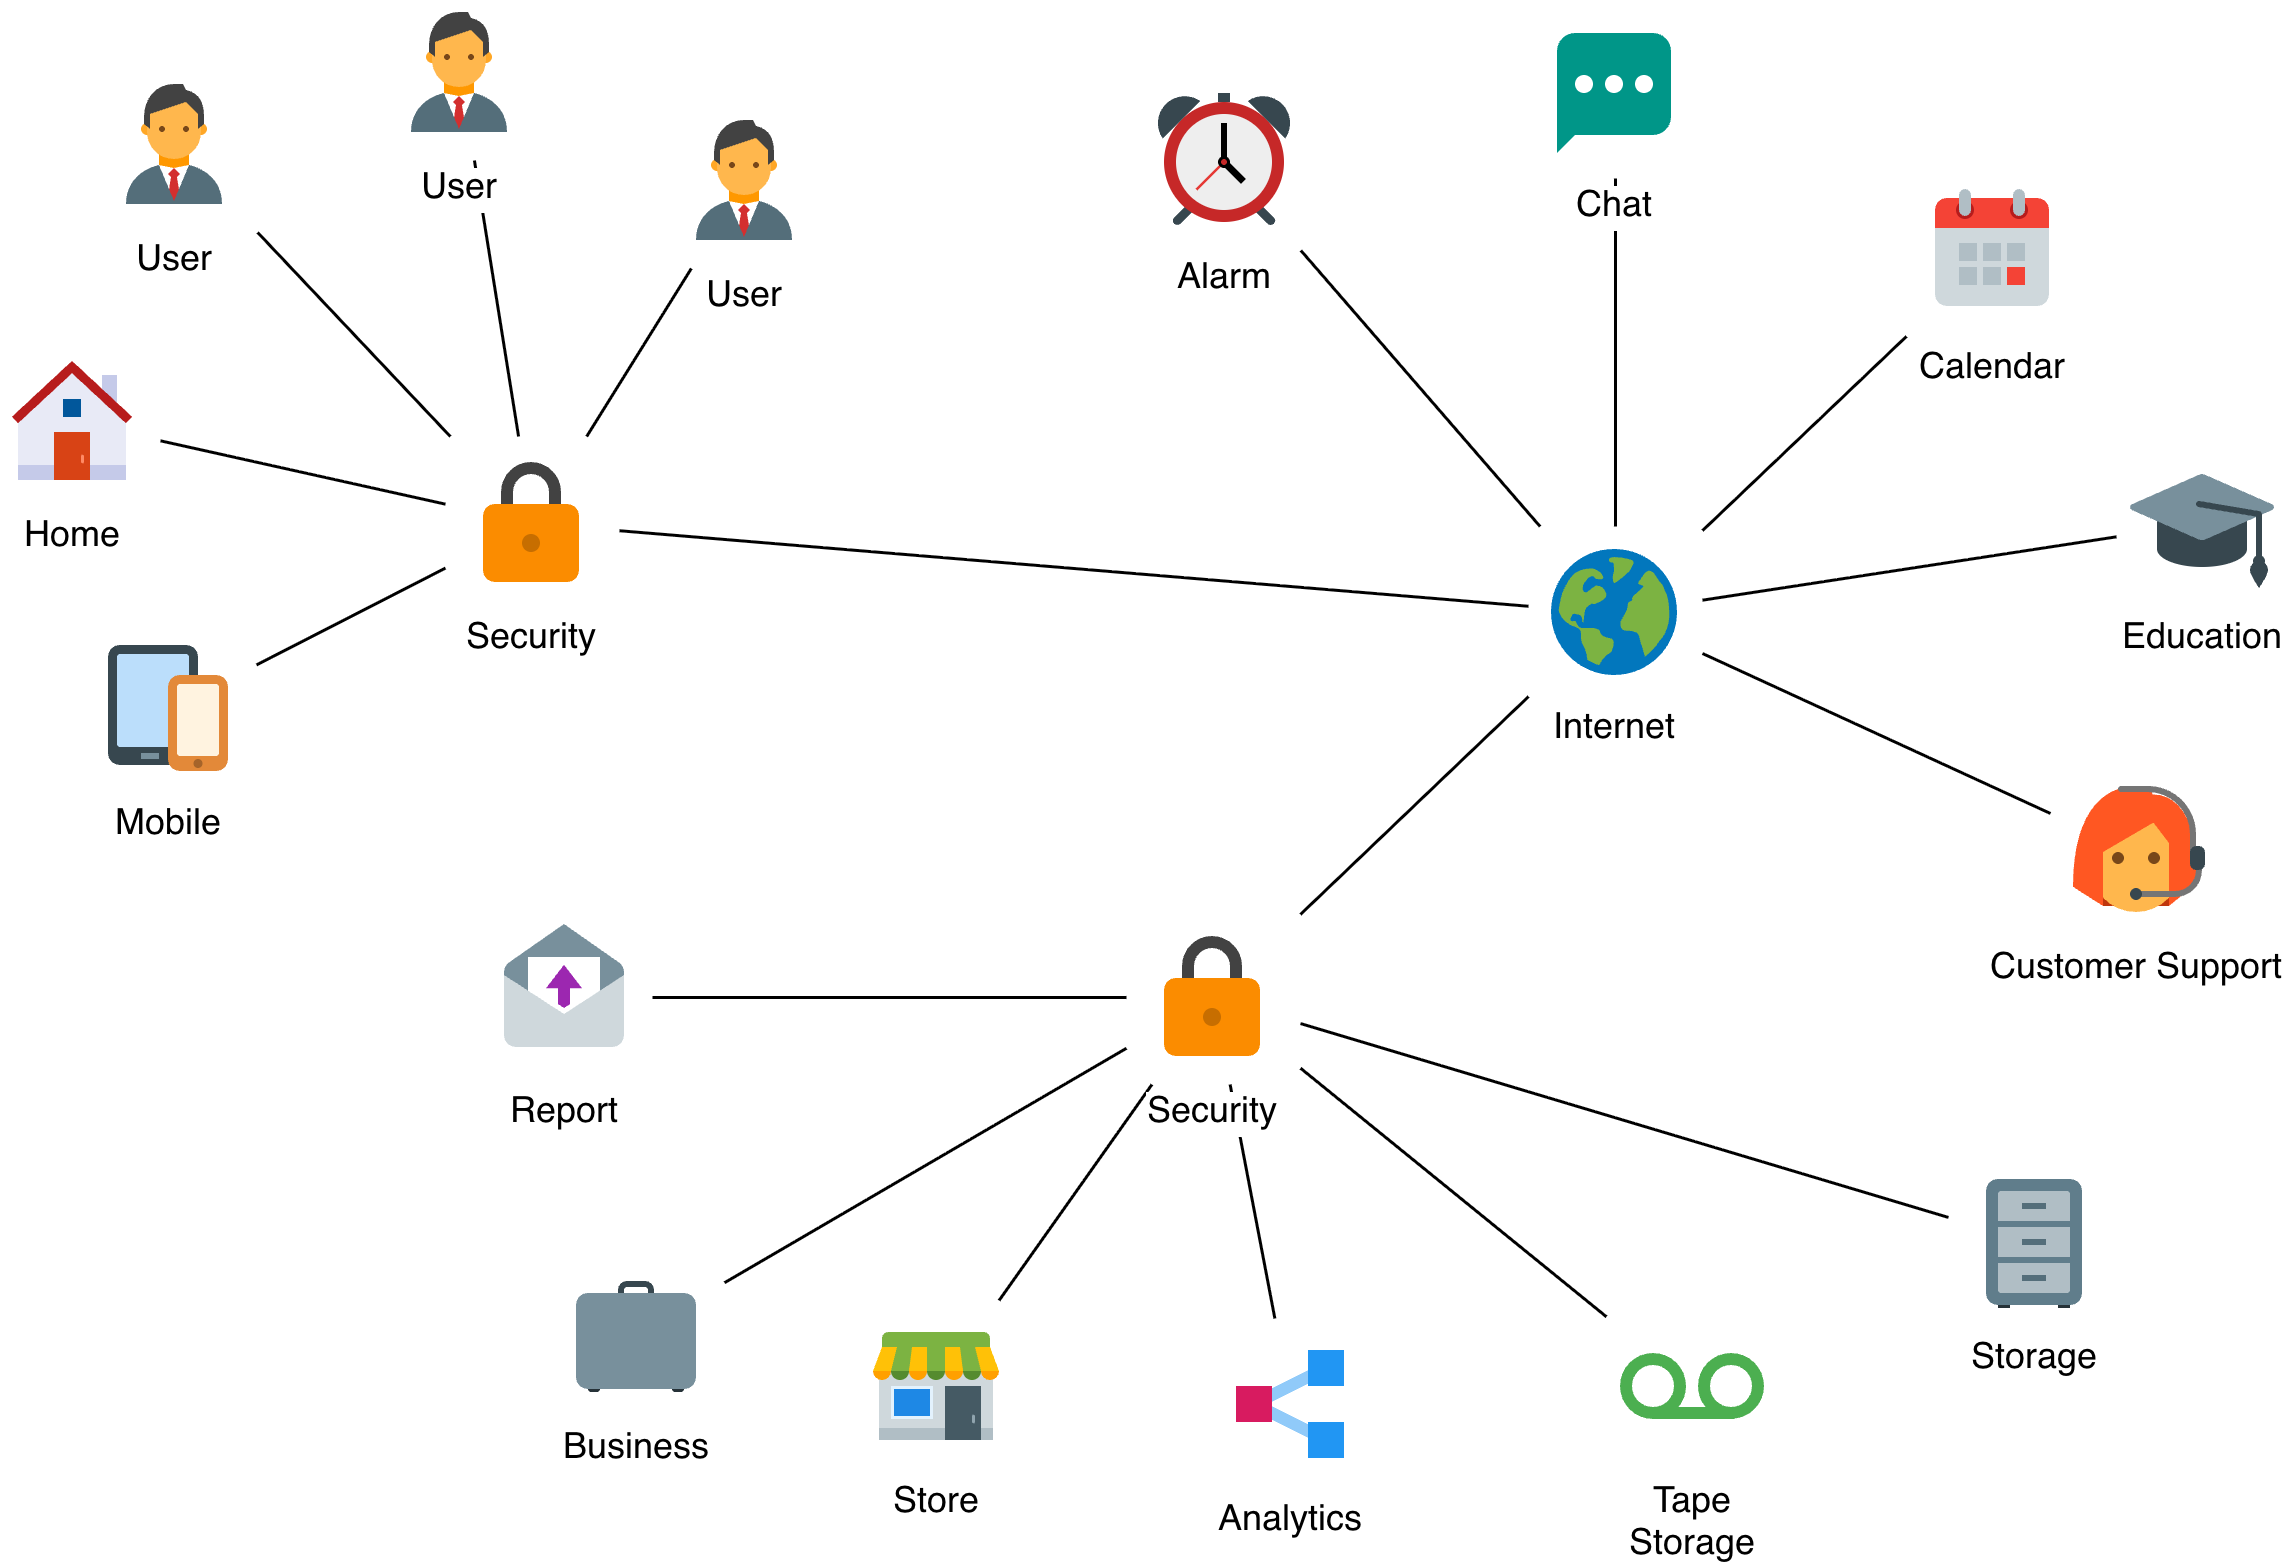
\includegraphics[width=0.7\textwidth]{gambar1.png}
	\caption{Contoh gambar jaringan}
	\label{gambar:jaringan}
\end{figure}


\subsubsection{Tabel}
Contoh tabel dapat dilihat pada Tabel \ref{tbl:harga1} dan \ref{tbl:harga2}. Tabel dan judulnya dibuat rata kiri dan judul tabel diletakkan di atas tabel. Usahakan tabel dapat ditulis dalam satu halaman, tidak terpotong ke halaman berikutnya.

\begin{table}[t] % pilihan opsi yang disarankan: t = top, b = bottom, h = here
  \begin{tabular}{ | p{2cm} | p{2cm} | p{3cm} |}
	\hline
	Nama 	& Satuan 		& Harga \\
	\hline
	Buku 	& Exemplar	& 25000 \\
	Komputer	& Unit		& 2500000 \\
	Pensil	& Buah		& 118900 \\
	\hline
	\end{tabular}
\caption{Tabel harga bahan pokok}
\label{tbl:harga1}
\end{table}

\begin{table}[h] % pilihan opsi yang disarankan: t = top, b = bottom, h = here
	\begin{tabular}{ | l | c | r | }
	\hline
	Nama 	& Satuan 		& Harga \\
	\hline
	Buku 	& Exemplar	& 25000 \\
	Komputer	& Unit		& 2500000 \\
	Pensil	& Buah		& 118900 \\
	\hline
	\end{tabular}
\caption{Tabel harga bahan sekunder}
\label{tbl:harga2}
\end{table}

\subsubsection{Rumus}
Contoh rumus matematika dapat ditulis seperti pada Persamaan \ref{eq:contoh1} di bawah ini. 
Penomoran persamaan diletakkan di sebelah kanan, dan rumus ditulis dalam mode \textit{display math}.
\begin{equation}
E = mc^2
\label{eq:contoh1}
\end{equation}

\subsection{Algoritma, Pseudocode, atau Kode}
Contoh penulisan algoritma atau pseudocode dapat ditulis seperti pada Kode \ref{alg:contoh1} di bawah ini. 
Gunakan paket \textit{listings} untuk menulis source code dalam bahasa pemrograman tertentu, seperti pada Kode \ref{lst:contoh1}. 


% -- Example of pseudocode and source code listing --
% -- Gunakan minipage agar listing tidak terpotong ke halaman berikutnya --
\begin{minipage}{\textwidth} 
\begin{lstlisting}[frame=lines, captionpos=t, caption={Contoh pseudocode}, label={alg:contoh1}]
ALGORITHM HelloWorld
   PRINT "Hello, World!"
END ALGORITHM
\end{lstlisting}
\end{minipage}

\begin{minipage}{\textwidth}
\begin{lstlisting}[language=Python, frame=single, caption={Contoh source code Python}, captionpos=t, label={lst:contoh1}]
def hello_world():
    print("Hello, World!")       
hello_world()
\end{lstlisting}
\end{minipage}


\section{Beberapa Kesalahan Penulisan yang Sering Terjadi}
\subsection{Penggunaan kata "di mana" atau "dimana"}
Banyak yang menuliskan kata "di mana" atau "dimana" sebagai pengganti kata "which" dalam bahasa Inggris. 
Padahal, penggunaan kata "di mana" atau "dimana" tidak tepat dalam konteks tersebut. Demikian juga untuk kata serupa, misalnya "yang mana".
Kata "di mana" atau "dimana" ini harus diganti dengan kata lain, seperti "dengan", "tempat", "yang", dan sebagainya tergantung kalimatnya.
Penjelasan lengkap dapat dilihat pada \autocite{BPBI}.

\subsection{Penggunaan kata "sedangkan" dan "sehingga"}

\begin{table}[htbp]
  \begin{tabular}{|c|c|c|}
  \hline
  Penggunaan kata & Salah & Benar \\ \hline
  sedangkan & \begin{tabular}[c]{@{}c@{}}Sedangkan sistem lama masih\\ digunakan oleh banyak pengguna.\end{tabular} & \begin{tabular}[c]{@{}c@{}}Sistem lama masih digunakan\\ oleh banyak pengguna,\\ sedangkan sistem baru belum siap.\end{tabular} \\ \hline
  sehingga & \begin{tabular}[c]{@{}c@{}}Sehingga sistem lama masih\\ digunakan oleh banyak pengguna.\end{tabular} & \begin{tabular}[c]{@{}c@{}}Sistem lama masih digunakan\\ oleh banyak pengguna sehingga\\ sistem baru belum siap.\end{tabular} \\ \hline
  \end{tabular}
  \caption{Contoh penggunaan kata "sedangkan" dan "sehingga"}
  \label{tbl:sedangkan_sehingga}
\end{table}

Kata "sedangkan" dan "sehingga" adalah kata hubung atau konjungsi. 
Konjungsi adalah kata atau ungkapan yang menghubungkan satuan bahasa 
(kata, frasa, klausa, dan kalimat). 
Konjungsi dapat dibagi menjadi konjungsi intrakalimat dan antarkalimat.  
Kata "sedangkan" menghubungkan dua klausa yang bersifat kontrasif, 
sedangkan "sehingga" menghubungkan dua klausa yang bersifat kausal. 
Dalam ragam formal, kata hubung “sedangkan” dan “sehingga” hanya dapat digunakan 
sebagai konjungsi intrakalimat sehingga kedua konjungsi itu \textbf{tidak dapat diletakkan pada awal kalimat}.
Selain itu, penggunaan kata "sedangkan" harus didahului oleh koma (,), sedangkan kata "sehingga" tidak perlu didahului oleh koma (,).
Contoh penggunaan yang benar dan salah dapat dilihat pada Tabel \ref{tbl:sedangkan_sehingga}.


\subsection{Penggunaan Istilah yang Tidak Baku}
Ada beberapa istilah yang sering digunakan dalam pembicaraan sehari-hari, tetapi tidak baku dalam penulisan ilmiah.
Beberapa istilah tersebut antara lain:
\begin{enumerate}
  \item analisa $\rightarrow$ analisis
  \item eksisting atau existing $\rightarrow$ yang ada atau saat ini
  \item bisnis proses $\rightarrow$ proses bisnis
  \item user $\rightarrow$ pengguna
  \item system $\rightarrow$ sistem
  \item database $\rightarrow$ basis data
  \item aktifitas $\rightarrow$ aktivitas
  \item efektifitas $\rightarrow$ efektivitas
  \item sosial media $\rightarrow$ media sosial
\end{enumerate}




% ============================================================================================
% BAB III ANALISIS MASALAH
% Pembagian subbab tidak rigid dan dapat bervariasi. Bab ini minimal berisi analisis kebutuhan
% fungsional dan nonfungsional, analisis berbagai alternatif solusi yang dapat ditawarkan, dan
% metode pemilihan solusi yang diusulkan.
% ============================================================================================
\chapter{ANALISIS MASALAH}
\section{Analisis Kondisi Saat Ini}
Menurut \textcite{laudon2020}, gambarkan terlebih dahulu model konseptual sistem yang ada saat ini. Model konseptual ini berisi berbagai komponen atau subsitem dan interaksi antarsubsistem tersebut. Setelah itu, berikan penjelasan tentang masalah yang ada pada sistem tersebut. Paragraf berikut berisi contoh penjabaran masalah sistem informasi fasilitas kesehatan untuk pasien \autocite{pressman2019}. 
\section{Analisis Kebutuhan}
\lipsum[4]
\subsection{Identifikasi Masalah Pengguna}
\lipsum[5]
\subsection{Kebutuhan Fungsional}
\lipsum[6]
\subsection{Kebutuhan Nonfungsional}
\lipsum[7]

\section{Analisis Pemilihan Solusi}
\subsection{Alternatif Solusi}
\lipsum[8]
\subsection{Analisis Penentuan Solusi}
\lipsum[9]

% ==========================================
% BAB IV DESAIN KONSEP SOLUSI
% ==========================================
\chapter{DESAIN KONSEP SOLUSI}
Ilustrasikan desain konsep solusi dalam bentuk model konseptual dan penjelasan secara ringkas, 
beserta perbedaannya dengan sistem saat ini. Ilustrasi harus dapat dibandingkan (\textit{before} and \textit{after}). 
Karena masih berupa proposal, bab ini hanya berisi gambar desain konsep solusi tersebut dan 
penjelasan perbandingannya dengan gambar sistem yang ada saat ini (yang tergambar di awal Bab III).

% ==========================================
% BAB V RENCANA SELANJUTNYA
% ==========================================
\chapter{RENCANA SELANJUTNYA}
Jelaskan secara detail langkah-langkah rencana selanjutnya, hal-hal yang diperlukan atau akan disiapkan, dan risiko dan mitigasinya, yang meliputi:
\begin{enumerate}
\item	Rencana implementasi, termasuk alat dan bahan yang diperlukan, lingkungan, konfigurasi, biaya, dan sebagainya.
\item	Desain pengujian dan evaluasi, misalnya metode verifikasi dan validasi.
\item	Analisis risiko dan mitigasi, misalnya tindakan selanjutnya jika ada yang tidak berjalan sesuai rencana.
\end{enumerate}


\backmatter

% ==========================================
% DAFTAR PUSTAKA
% ==========================================
\printbibliography[title={DAFTAR PUSTAKA}]

% ==========================================
% LAMPIRAN (optional)
% ==========================================
\appendix

\chapter{LAMPIRAN A: SOURCE CODE}

\chapter{LAMPIRAN B: HASIL SURVEI}


\end{document}
 